\documentclass{article}
\usepackage[utf8]{inputenc}
\usepackage[francais]{babel}
\usepackage[T1]{fontenc}
\usepackage{lmodern}
\usepackage{ifpdf}
\usepackage{graphicx}
\usepackage{geometry}
\renewcommand{\familydefault}{\sfdefault}

\geometry{hmargin=50pt, vmargin=50pt}

\title{Cahier des charges : Tableau virtuel interactif}
\author{Baptiste Saleil \and Geoffrey Mélia \and Julien Pagès \and Kevin Bollini}
\date{\today}
\ifpdf
	\pdfinfo 
	{
		/Author (bsaleil,gmelia,jpages,kbollini)
		/Title (Rapport de projet)
		/Subject (Tableau virtuel interactif)
		/Keywords ()
		/CreationDate (\today)
	}
\fi

\begin{document}
	% Page de titre
	\maketitle
	\thispagestyle{empty}
	\newpage
	
	% Sommaire
	\tableofcontents
	\newpage
	
	\section{Introduction}
		\subsection{Fonctionnement général}
			Le but de l'application est de simuler une écriture ou un dessin sur un tableau virtuel. Ceci en se basant 
		sur une reconnaissance de mouvements via une webcam.
		\subsection{Finalités}
			Pour ce projet universitaire, l'objectif est d'obtenir un produit qui soit réellement utilisable.
La finalité est donc d'avoir la possibilité de pouvoir utiliser rapidement l'application avec un étalonnage simple et rapide.\\
De plus l'intérêt est également d'avoir une application utile qui peut par exemple être utilisée dans le cadre d'un cours,
pour rapidement dessiner un schéma et l'exporter et le sauvegarder ensuite. \\
\subsection{Choix stratégiques}
			Pour mener à bien ce projet, nous avons choisi de le découper.
			Ce découpage nous permettra de mieux nous organiser, de mieux répartir les tâches, et donc de fournir un travail plus efficace, même sur le long terme.
			\subsubsection{Librairie - Application}
			Notre premier choix consiste à découper notre projet en deux projets bien distincts, une librairie de suivi de mouvements, et une application graphique. \\ \\
			Ce choix représente plusieurs intérêts : \\
			\begin{itemize}
				\item{Premièrement, ce découpage permet de bien différencier les tâches, le développement de la librairie requiert des connaissances en traitement d'images pour tracer des couleurs/objets, appliquer des filtres, manipuler les images, etc... ce qui correspond parfaitement à la formation de deux membres du groupe. (Formation IMAGINA Université Montpellier 2). Le développement de l'application, lui, requiert des connaissances en génie logiciel, pour l'architecture de l'application, en IHM, pour la réalisation de l'interface (logicielle et gestuelle), ou encore en réseau pour la mise en place de l'architecture client/serveur. Ces différents points correspondent également parfaitement à la formation des deux autres membres du groupe. (Formation AIGLE Université Montpellier 2). Ainsi, les tâches peuvent bien se répartir en fonction des connaissances et spécialités de chacun.} \\
				\item{Deuxièmement, l'intérêt de ce découpage est d'avoir deux projets complètement indépendants. En effet, la librairie sera développée d'un côté et permettra d'offrir un bon nombre de fonctionnalités de suivi ou manipulation d'image. L'application, elle, se chargera d'utiliser les fonctionnalités de traitement d'image de la librairie en ajoutant une interface, une couche réseau, une connexion aux webcam, la récupération du flux, etc...
				La librairie et l'application sont donc deux projets développés en parrallèles et très modulaires, notre application peut très bien utiliser une autre librairie de traitement d'image, et la librairie peut très bien être utilisée par d'autres application qui offriraient des fonctionnalités totalement différentes de la notre.}
			\end{itemize}
				\subsubsection{Différentes étapes}
				Notre deuxième choix à été de découper le projet en plusieurs étapes. Arrivés en Master 1, nous avons maintenant quelques projets à nos actifs et savons maintenant comment éviter certaines erreurs. L'objectif final du projet est assez haut, ce choix d'étapes nous permet donc d'avoir un premier objectif accessible, puis d'ajouter des fonctionnalités à la librairie, et à l'application petit à petit pour franchir les étapes et s'approcher au maximum de nos objectifs. On pourrait par exemple se fixer les étapes qui suivent : \\
				\begin{itemize}
					\item{Prototype fonctionnel avec côté librairie une reconnaisance basique de forme ou mouvement, et côté application une interface basique permettant d'accéder à la webcam, d'appeler la librairie, de dessiner sans personnalisation, ainsi qu'une ébauche du module réseau. Ce prototype permettra de poser les bases de l'architecture de l'application et de la librairie.}
					\item{Ajout d'algorithmes de reconnaissance et de nouvelles méthodes de reconnaissance pour la librairie, et amélioration du module réseau (définition du protocole, application serveur fonctionnelle, gestion des paquets, etc...)}
					\item{Optimisation des algorithmes de trace et optimisation des méthodes. Ajout de l'interface gestuelle et personnalisation du dessin.}
					\item{Finalisation du code, préparation d'une utilisation en production. Compilation dynamique de la librairie, création de paquets linux (.deb,...) compilation sur plusieurs systèmes d'exploitation.}
				\end{itemize}
	\section{Contexte}
		\subsection{Faisabilité}
		Notre groupe ayant lui-même proposé ce sujet, celui-ci s'accorde parfaitement à nos formations et spécialités. Le choix de ce sujet a donc été réalisé en fonction de nos expériences, savoir-faire et affinités.\\
Ce projet s'inscrivant dans le cadre d'un TER de notre formation, l'étude de la faisabilité n'incluera pas certains critères comme l'étude de marché, le contexte économique ou le besoin réel. Nous allons nous concentrer notamment sur les compétences techniques et de gestion. Pour les parties financement et analyse des coûts, il va sans dire que nous ne disposons d'aucun financement et n'allons utiliser que des outils gratuits. \\
Comme dit précédemment, le projet est décomposé en deux parties majeures que sont l'application et la librairie (dont les contenus seront détaillés dans des sections qui leur sont propres).
			\paragraph{Application :\\}
L'application doit exploiter le plus efficacement possible la librairie de reconnaissance. Nous voulons donc mettre en place un étalonnage de l'objet à suivre le plus précisément possible. Le projet doit ensuite être exploitable et utile, nous devons donc mettre en place un certain nombre d'outils tels que la possibilité de gommer, changer de forme, de couleur etc. 
Un module réseau est aussi prévu pour une utilisation concurrente et synchronisée. Et bien sûr la fonctionnalité clé de l'application est le tableau virtuel, qui devra donc être exploitable et le dessin devra être fidèle aux mouvements reconnus.
			\paragraph{Librairie :\\}
				Cette partie du développement a pour objectif de fournir un ensemble de fonctions permettant la reconnaissance et le traçage d'un objet à partir d'un flux vidéo, ou plus généralement d'une suite d'images. Un certain nombre de librairies existantes proposent des moyens d'accéder à cet objectif, notamment grâce à des outils de reconnaissance de forme, de suivi de modèle ou d'évalutation de composantes connexes. Le travail consiste donc à tirer partie de ces bibliothèques en les associant de manière à proposer des méthodes efficaces et simples à utiliser. Cela implique une bonne connaissance des outils existants, de leur compréhension et de leur utilisation conjointes.
		\subsection{Existant}
		La vision par ordinateur et particulièrement le traçage virtuel d'objets, sont des domaines connus et pour lesquels il existe de nombreux travaux. Nous pouvons nous inspirer de certains de ces travaux afin de proposer des fonctionnalités plus pertinentes, éviter certains écueuils ou plus directement utiliser des outils existants comme la librairie OpenCV.\\
			\begin{itemize}
				\item Exemples dans le jeux vidéo : Kinect, Eye-toy, CamSpace (techniques pour l'IHM, par exemple, mouvements continus ou immobilité sur une zone).
				\item Exemples issus de thèses et de projets de recherche (techniques de programmations).
			\end{itemize}
		\subsection{Ressources}
		Nous utiliserons en première partie du projet essentiellement des articles de recherches pour découvrir et comprendre différentes problématiques liées à l'IHM naturelle (mouvements du corps) ainsi que des recherches autour de l'imagerie numérique. \\ Ensuite nous utiliserons des ressources plus concrètes comme des livres de programmation (OpenCV, documentation).
		
		\paragraph{Documents de recherches}
			\begin{itemize}
			\item \it{Real-time viewpoint-invariant hand localization with cluttered backgrounds} \\
			Enver Sangineto, Marco Cupelli.
			\begin{verbatim}
			http://www.sciencedirect.com/science/article/pii/S026288561100120X
			\end{verbatim}
			\item \it{Vision par ordinateur pour l’interaction homme-machine fortement couplée}\\
			Thèse de françois Bérard sur un sujet proche avec beaucoup d'informations
			\begin{verbatim}
			http://hal.inria.fr/docs/00/04/61/56/PDF/tel-00004804.pdf
			\end{verbatim}
			\item \it{Defining Search Areas to Localize Limbs in Body Motion Analysis} \\
			Thomas Foures, Philippe Joly.
			\item \it{Indexation de la vidéo par le costume.}\\ 
			Thèse de doctorat, Université Paul Sabatier Toulouse, Gaël Jaffré.
			\begin{verbatim}
			http://www.irit.fr/recherches/SAMOVA/pageautomatic-character-labelling-in-videos.html
			\end{verbatim}
			\end{itemize}
			
		\paragraph{Documents de programmation}
			\begin{itemize}
			\item \it{Vision par ordinateur : Outils fondamentaux} \\
			Radu HORAUD (CNRS) et Olivier MONGA (INRIA)
			\begin{verbatim}
			http://hal.archives-ouvertes.fr/docs/00/59/00/49/PDF/VO-HoraudMonga.pdf
			\end{verbatim}
			\item Learning Open CV \\
			 Gary Bradski et Adrian Kaehler
			\item Open Cv 2 Computer Vision Application Programming Cookbook\\
			Robert Laganière
			\end{itemize}
			
	\section{Analyse et conception}
		\subsection{Organisation}
		Le projet se déroulera autour de trois dates clés:
			\begin{itemize}
				\item 2 Mars 2012 : Bilan de mi-parcours.
				\item mi-avril 2012 : Pré-soutenance au LIRMM.
				\item 27 Avril 2012 : Bilan de pré-soutenance.
				\item 14 Mai 2012 : Rendu complet du projet.
			\end{itemize}
			Nous devons donc fixer nos objectifs en fonction de celles-ci, en essayer de réaliser la première étape, le prototype fonctionnel, aux alentours de la première date.
		
			Nous utiliserons donc un planning, pour avoir une vision globale des grandes lignes du projet, et des réunions fréquentes pour se synchroniser. 
		\subsection{Planning}
			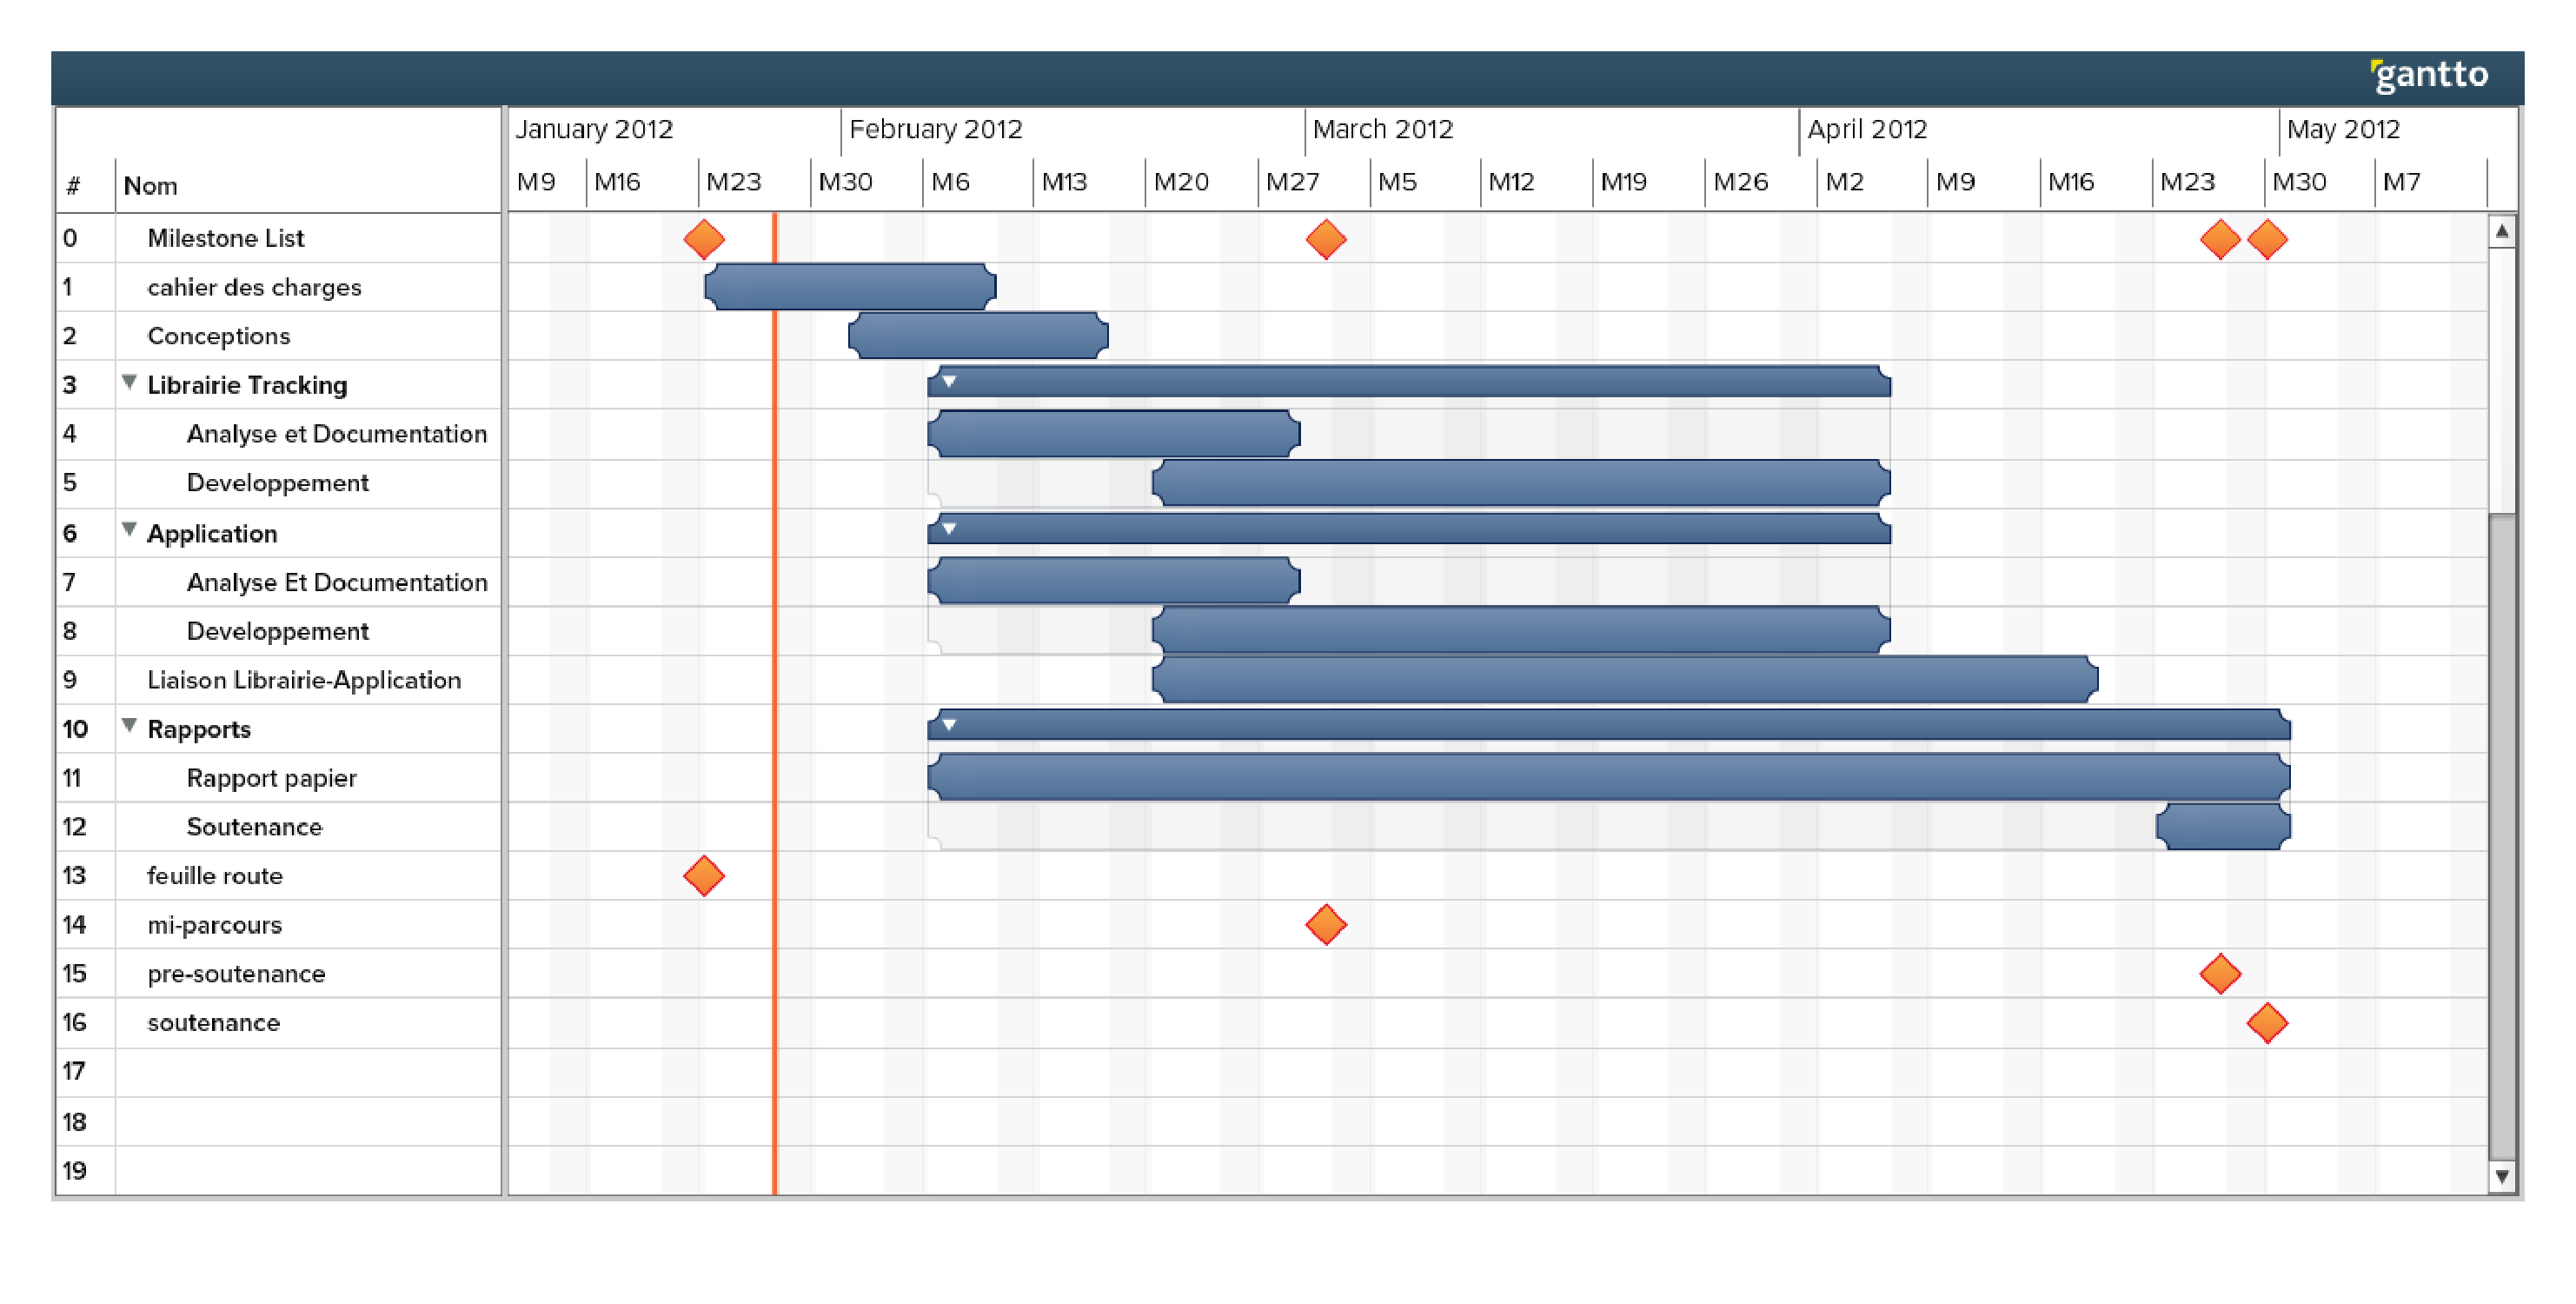
\includegraphics[scale=0.3]{retroplanning.pdf}
			\begin{center}
			\it{rétro-planning}
			\end{center}
			
		Deux équipes tranvailleront en parallèle  : une pour la librairie de reconnaissance, et l'autre à la partie logicielle et interface homme-machine. \\
		Une première phase de conception, pour faire l'UML et bien penser l'application sera importante en temps. 
		La conception doit permettre d'ajouter des modules très facilement (comme les fonctionnalités réseaux, la personnalisation des formes, couleurs...). \\
		Ensuite le développement devra être incrémental et avoir des étapes avec des résultats visibles et exploitables avant d'ajouter d'autres fonctionnalités. \\ 
		\subsection{UML}
		% TODO : à finir
		Tout d'abord nous devons évaluer les fonctionnalités finales de l'application et ne pas les perdre de vue, elles sont donc décrites dans les cas d'utilisations suivants. \\
			\begin{center}
			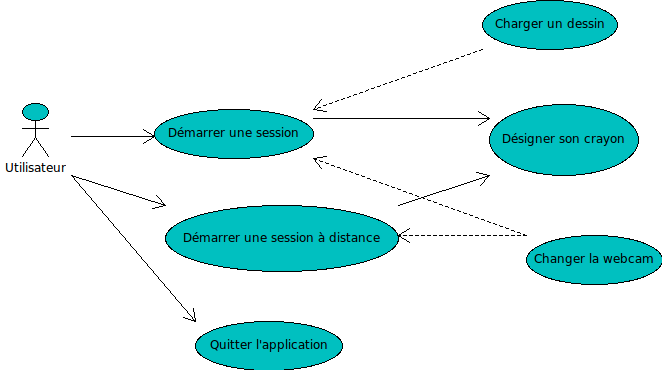
\includegraphics[scale=0.7]{../uml/Accueil.png} \\
			\it{Cas d'utilisation de l'accueil de l'application}
			\end{center}
			
			\begin{center}
			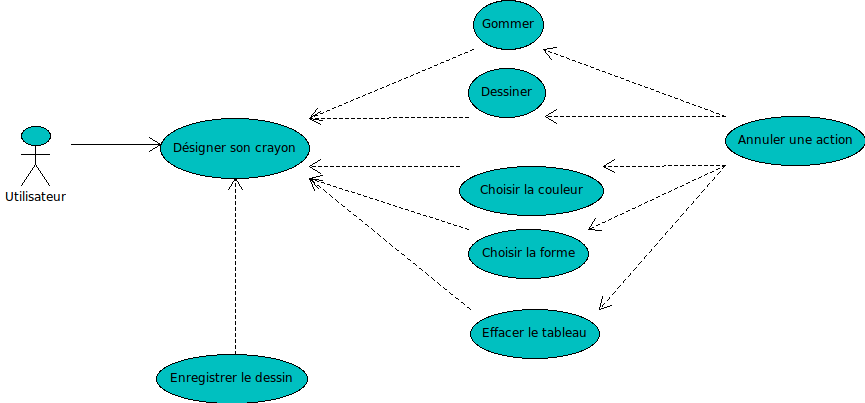
\includegraphics[scale=0.7]{../uml/Dessin.png} \\
			\it{Cas d'utilisation de l'accueil de l'application}
			\end{center}
\newpage
	\section{Librairie}
		\subsection{Fonctionnalités}
			Le but de cette librairie est de fournir des fonctions permettant le repérage et le suivi d'un objet en particulier à partir d'images. 
			L'idée serait donc d'avoir dans la librairie un maximum de fonctions de traçage différentes, de la plus lente et précise à la plus rapide et permissive, de manière à adapter la complexité en fonction du degré de précision requis pour notre traitement. \\
			On peut alors imaginer deux classes de fonctions, des plus basiques réalisant un tracking intuitif (sans mémoriser d'informations sur l'objet suivi par ex.) aux plus perfectionnées effectuant un repérage préliminaire pour connaitre l'objet.
			Le repérage devra permettre à partir d'une image et d'une position de reconnaître et d'isoler un objet. Cette étape permettra de récupérer un certain nombre de caractéristiques sur l'objet qui permettront ensuite de le suivre, comme par exemple sa couleur ou sa taille. \\
Dans un premier temps, nous implémenterons une fonction basique de suivi par couleur, retournant la position polaire de l'objet sur l'image. \\
Dans un second temps, nous essayerons d'inclure à la librairie des fonctions de détection d'actions permettant par exemple de signaler que l'on écrit. 
		\subsection{Architecture}
			Architecture de la librairie 
			\begin{itemize}
				\item Fonctions simples : On trace une forme ou une couleur, sans apprentissage, à partir de deux images et d'une position.
				\item Fonctions "intelligente" : On commence par recueillir des informations (forme, taille, ancienne localisation ou couleur par exemple) sur l'objet tracé que l'on conserve ensuite    
				\item Fonctions de détection d'actions (Mouvement/transformation signifiant une action. Par exemple, main qui se ferme pour clic)
			\end{itemize}
			L'objectif final serait de fournir cette librairie sous forme de bibliothèque dynamique d'abord au format UNIX .so et éventuellement en .dll pour windows. 
		\subsection{Outils}
			Nous utiliserons le langage C/C++ et la librairie OpenCV pour le développement de la librairie, qui sera elle-même destinée à C.
Notre choix s'est porté sur ce langage pour différentes raisons :
		\begin{itemize}
			\item Nous souhaitons utiliser la librairie OpenCV qui à été initialement créée pour le langage C.
			\item L'application sera elle aussi faite en C++.
		\item C'est le langage que nous connaissons et affectionnons le plus.
			\end{itemize}
			Nous avons décidé d'utiliser OpenCV car c'est une librairie puissante, très bien documentée et fortement orientée sur la vision par ordinateur. \\
		\subsection{Étapes}
			Détail des étapes avec fonctionnalités pour chacune d'elle.
	\section{Application}
		\subsection{Fonctionnalités}
		L'application doit permettre en premier lieu de faire rapidement un schéma ou écrire quelques phrases
et de le sauvegarder : ce qui n'est pas possible avec un tableau conventionnel. \\ 			
		Dans l'optique d'obtenir une application réellement fonctionnelle, permettra de dessiner 
et d'écrire sur le tableau virtuel avec une interface Homme-Machine naturelle. \\

		\begin{itemize}
			\item L'exportation du dessin ou de l'écriture vers un format pdf, ou image
			\item Une gomme permettant d'effacer	
			\item Un module réseau pour faire un travail collaboratif avec l'application
			\item Plusieurs formes de pinceaux avec plusieurs couleurs
		\end{itemize}

		\subsection{Architecture}
		% TODO : présenter l'architecture, avec diagramme des "boîtes"
			Architecture de l'application
		\subsection{Outils}
			Nous utiliserons des librairies pour accélérer le développement de l'application, et donc d'obtenir plus 
rapidement un résultat abouti.
		L'application contient une interface graphique, il nous faut donc une librairie pour cela :
		notre choix s'est porté sur Qt, pour plusieurs raisons : 
		\begin{itemize}
			\item La librairie est très puissante et complète, avec une bonne documentation
			\item Elle est multi-plateformes
			\item C'est une librairie que nous connaissons déjà un peu, cela réduit donc le temps passer à se former dessus
			\item C'est une librairie essentiellement C++, ce qui s'adapte au langage choisi pour l'application, et pour la librairie
		\end{itemize} \ \\
Nous utiliserons également QtDesigner pour nous assister dans la création de l'interface graphique (placement des éléments...). \\
		
OpenCV nous servira également pour accéder à la webcam (ou aux webcams). De plus cette librairie capturera des images et les enverra à la librairie pour le traitement. Cette partie sera bien sûr recouverte par une partie écrite en C++ avec Qt pour lister les webcams disponibles par exemple. \\

		Le développement se fera complètement sous Linux, avec à terme des essais sur d'autres systèmes d'exploitation pour
porter l'application sous ces systèmes. \\ 

		\subsection{Étapes}
		% TODO 
			Détail des étapes avec fonctionnalités pour chacune d'elle.
	\section{Conclusion}
	% TODO 	
		Conclusion (1 ou 2 paragraphe ?)
	
\end{document}

